
\documentclass[20pt]{beamer}

\usepackage[ngerman,english]{babel}
\usepackage{tikz}
\usepackage[normalem]{ulem}
\geometry{paperwidth=10in, paperheight=7.5in}
\usepackage{animate}

\usepackage[utf8]{inputenc}

\usepackage[mpidr]{./mpidr/beamerthemeMPIDR}


%%%%%%%%%%%%%%%%%%%%%%%%%%%%%%%%%%%%%%%%%%%%%%%%%%%%%%%%%%%%%%%%%%%%%%%%%%%%%%
% Title Page
%%%%%%%%%%%%%%%%%%%%%%%%%%%%%%%%%%%%%%%%%%%%%%%%%%%%%%%%%%%%%%%%%%%%%%%%%%%%%%%

\title[HLE, mortality and morbidity]{~~~Healthy Life Expectancy,\\~~~ Mortality,
\\~~~and Age Prevalence of Morbidity}
%\hspace{10cm}
%\small
\subtitle{Alyson van Raalte, Tim Riffe}
%\institute[PAA 2016]{MPIDR, Rostock, Germany}
%\date[]{\scriptsize April 2, 2016}

%%	the institute's logo
\renewcommand{\mylogo}{\includegraphics[width=4.7in]{mpidr_logo_colour_en}}
\usepackage{color}
\definecolor{mygray}{rgb}{0.8,0.8,0.8}

\defbeamertemplate{description item}{align left}{\insertdescriptionitem\hfill}
%%	should be the very last package to be loaded
\usepackage{hyperref}

\begin{document}
%%	titlepage - fixed frame:
%%	========================

\begin{frame}
	\titlepage
\end{frame}

%%%%%%%%%%%%%%%%%%%%%%%%%%%%%%%%%%%%%%%%%%%%%%%%%%%%%%%%%%%%%%%%%%%%%%%%%%%%%%%
\section{Introduction}
%%%%%%%%%%%%%%%%%%%%%%%%%%%%%%%%%%%%%%%%%%%%%%%%%%%%%%%%%%%%%%%%%%%%%%%%%%%%%%%

%%%%%%%%%%%%%%%%%%%%%%%%%%%%%%%%%%%%%%%%%%%%%%%%%
\begin{frame}{Expected life years with disability (DLY)} 
\begin{itemize}[<+->]
\item Most often measured by Sullivan method
\item DLY is sum product of lifetable survival $L_x$ and morbidity age-specific
prevalence $\pi_x$
\item DLY can change because of changes in $L_x$ or $\pi_x$
\end{itemize}
\end{frame}
%%%%%%%%%%%%%%%%%%%%%%%%%%%%%%%%%%%%%%%%%%%%%%%%%
\begin{frame}{But what is $\pi_x$ exactly?}
\begin{itemize}[<+>]
\item Disability prevalence at each age
\item Stock variable: slow to react to abrupt health innovations since it depends on past cohort experiences with sickness (Barendregt et al. 1994)
\item Prevalence can vary by age, time-to-death, lifespan, or combinations of
these things.
\item This complicates comparisons of period DLY (or HLE) across
populations with different mortality.
\item Since $\pi_x$ changes across mortality regimes, attributing
between-population differences in DLY to mortality and morbidity is problematic.
\end{itemize}
\end{frame}
%%%%%%%%%%%%%%%%%%%%%%%%%%%%%%%%%%%%%%%%%%%%%%%%%


%%%%%%%%%%%%%%%%%%%%%%%%%%%%%%%%%%%%%%%%%%%%%%%%%%
\section{Morbidity as a function of time to death}
%%%%%%%%%%%%%%%%%%%%%%%%%%%%%%%%%%%%%%%%%%%%%%%%%%

%%%%%%%%%%%%%%%%%%%%%%%%%%%%%%%%%%%%%%%%%%%%%%%%%%%%%%%%%%%%%%
\begin{frame}{A simple illustration}
\begin{center}
 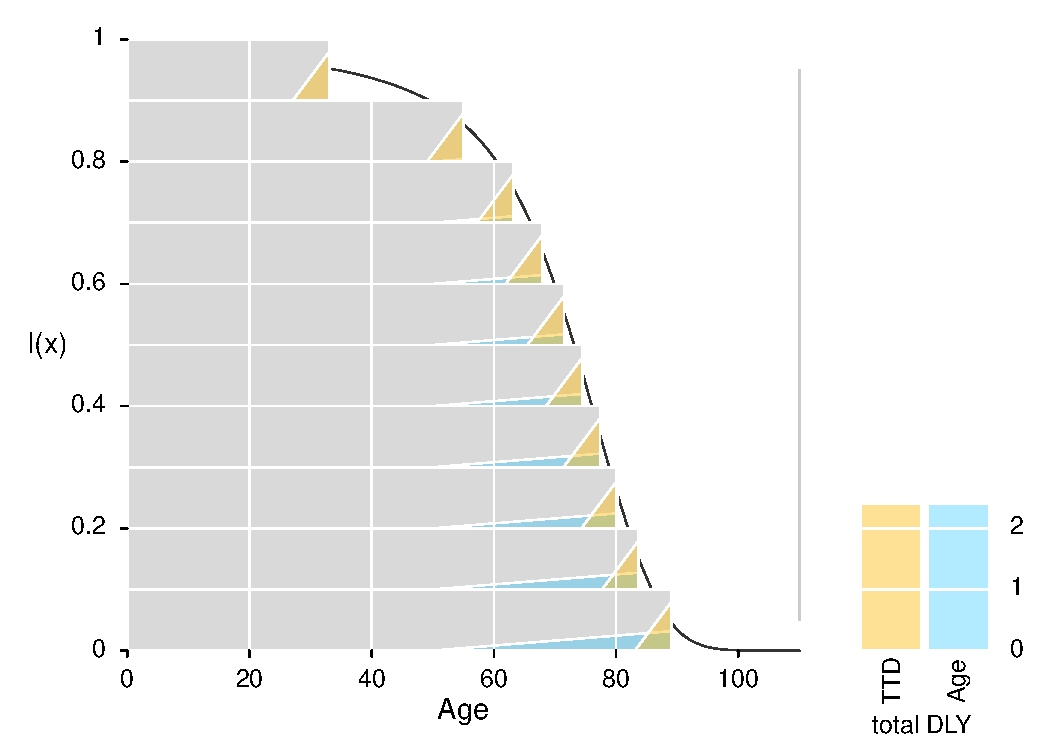
\includegraphics[width=\linewidth]{Figures/Japan1970.pdf}
 %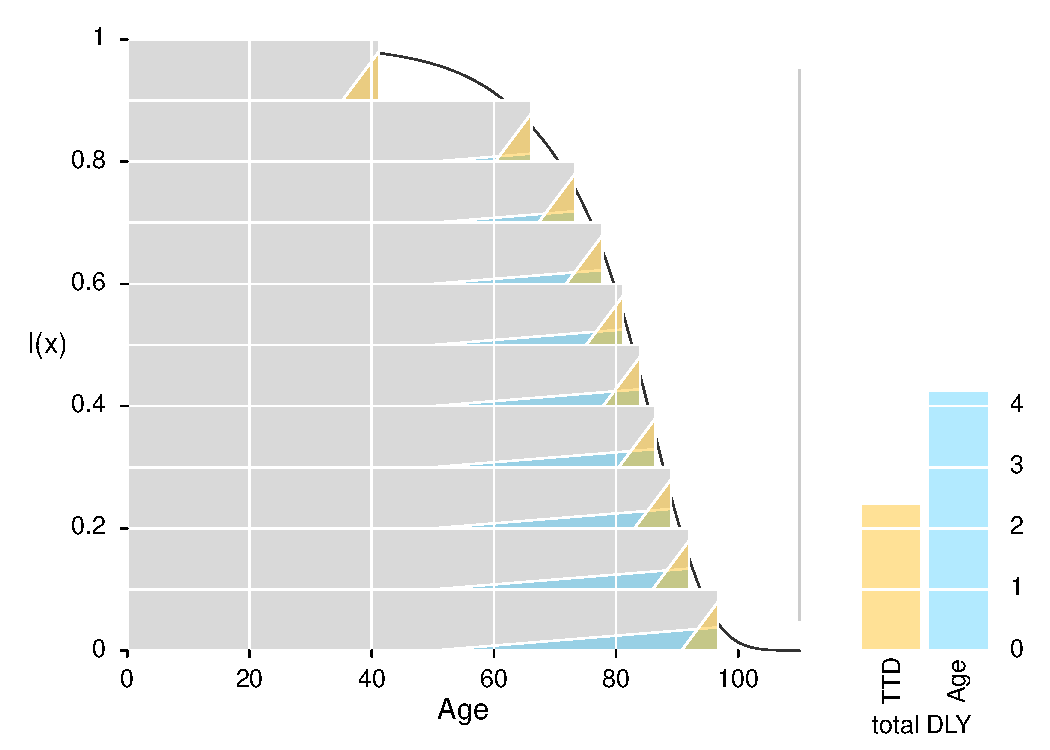
\includegraphics[width=.5\linewidth]{Figures/Japan2010.pdf}
\end{center}
\end{frame}

\begin{frame}{A simple illustration}
\begin{center}
 %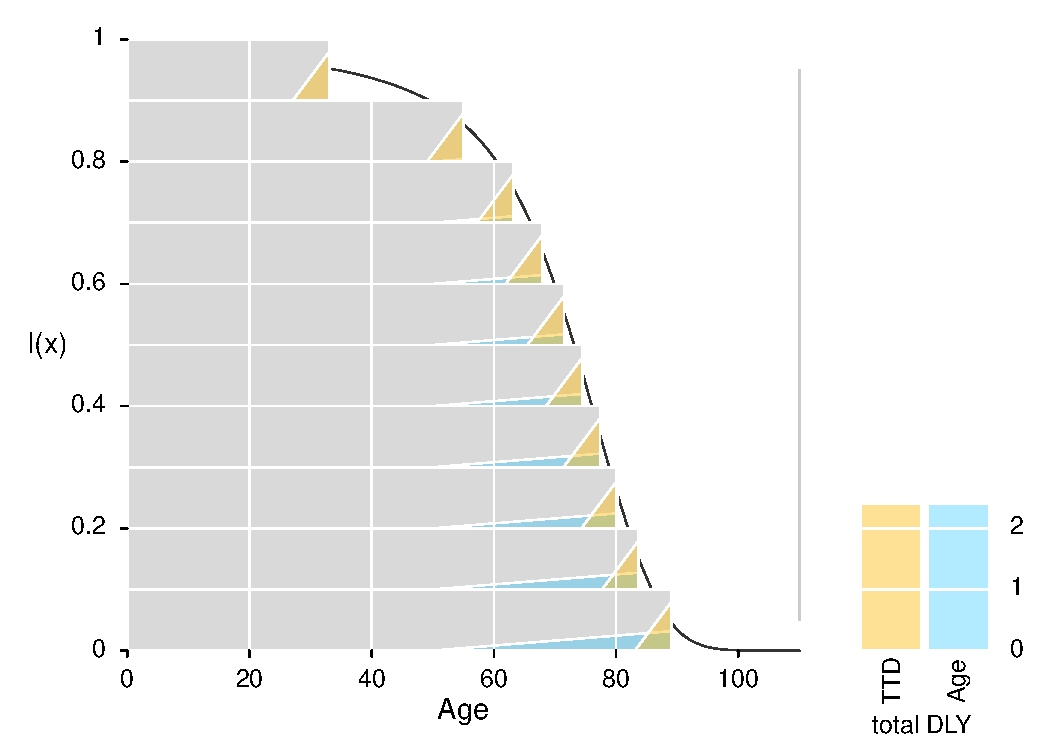
\includegraphics[width=.5\linewidth]{Figures/Japan1970.pdf}
 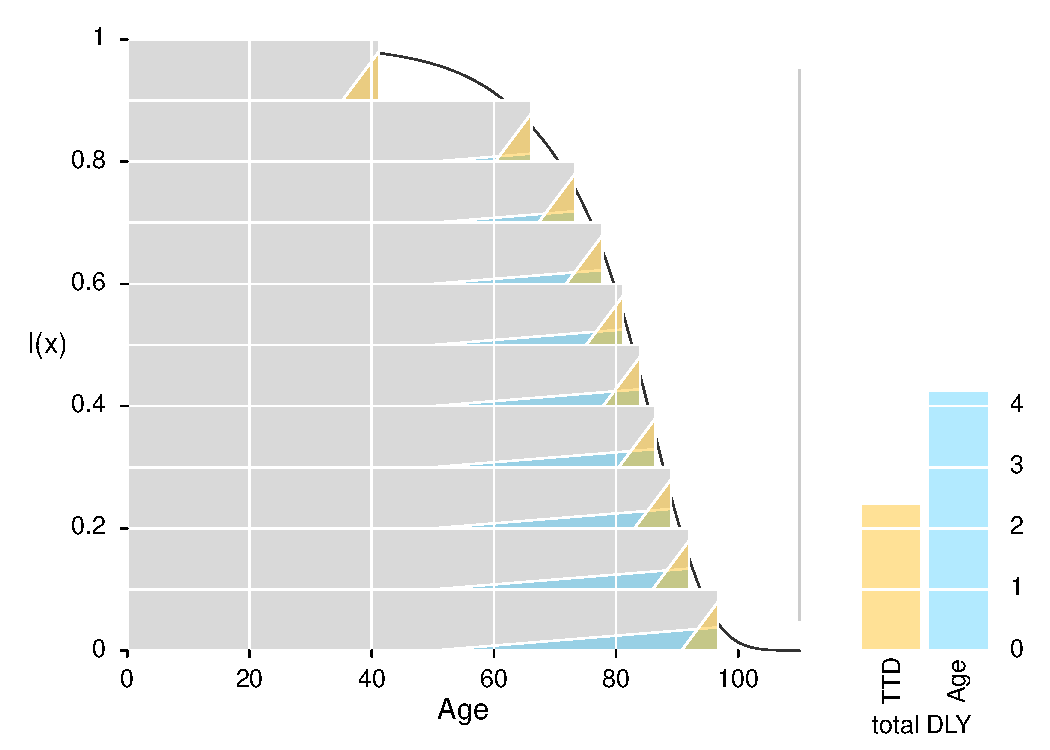
\includegraphics[width=\linewidth]{Figures/Japan2010.pdf}
\end{center}
\end{frame}

%%%%%%%%%%%%%%%%%%%%%%%%%%%%%%%%%%%%%%%%%%%%%%%%%%%%%%%%%%%%%%
%%%%%%%%%%%%%%%%%%%%%%%%%%%%%%%%%%%%%%%%%%%%%%%%%%%%%%%%%%%%%%%%%%%%%%%%%%%%%%%%%%%%%%%%%%%%%%%
\begin{frame}{Disablity broken down by age and time to death}{}
\begin{center}
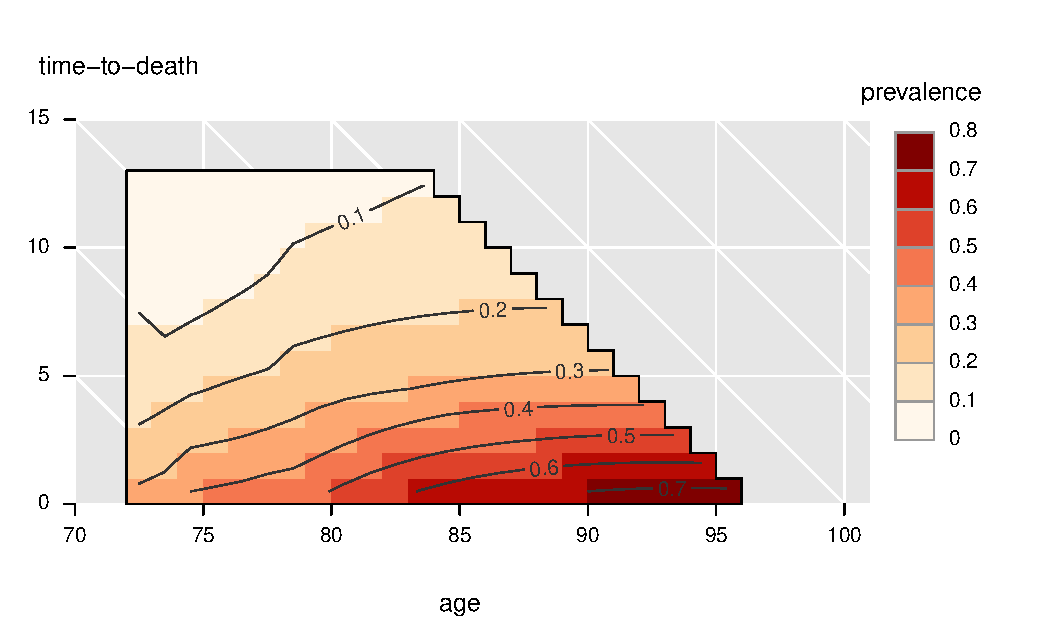
\includegraphics[scale=1.2]{Figures/IADL1_Males.pdf}
\\
\small Proportion of USA
males from the 1915-1919 cohort with at least 1 of 5 IADLs
\end{center}
\end{frame}

\begin{frame}{Disablity broken down by age and time to death}{}
\begin{center}
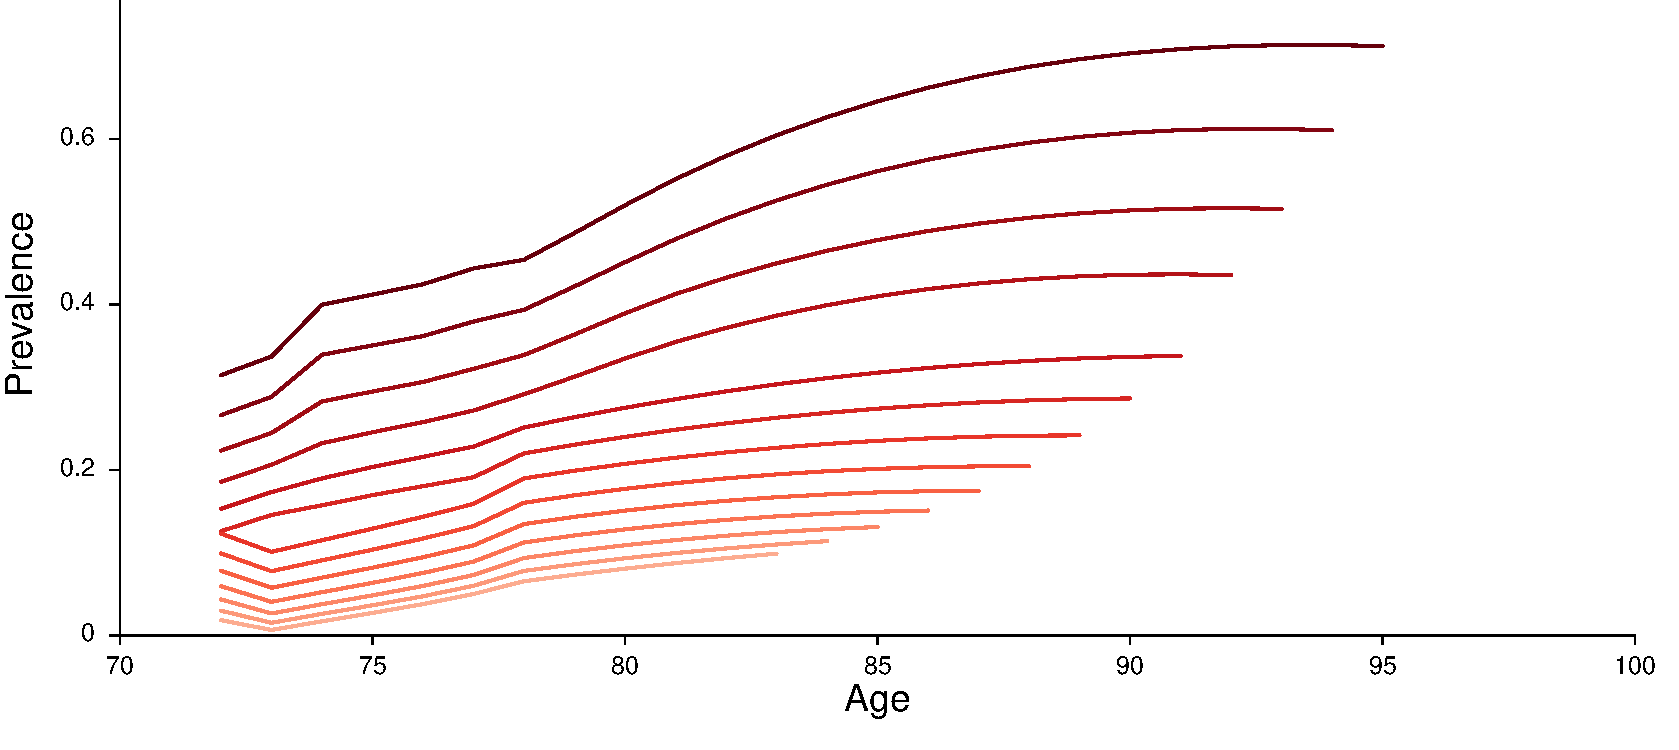
\includegraphics[scale=.8]{Figures/IADLagelines.pdf}
\end{center}
\end{frame}

\begin{frame}{Disablity broken down by age and time to death}{}
\begin{center}
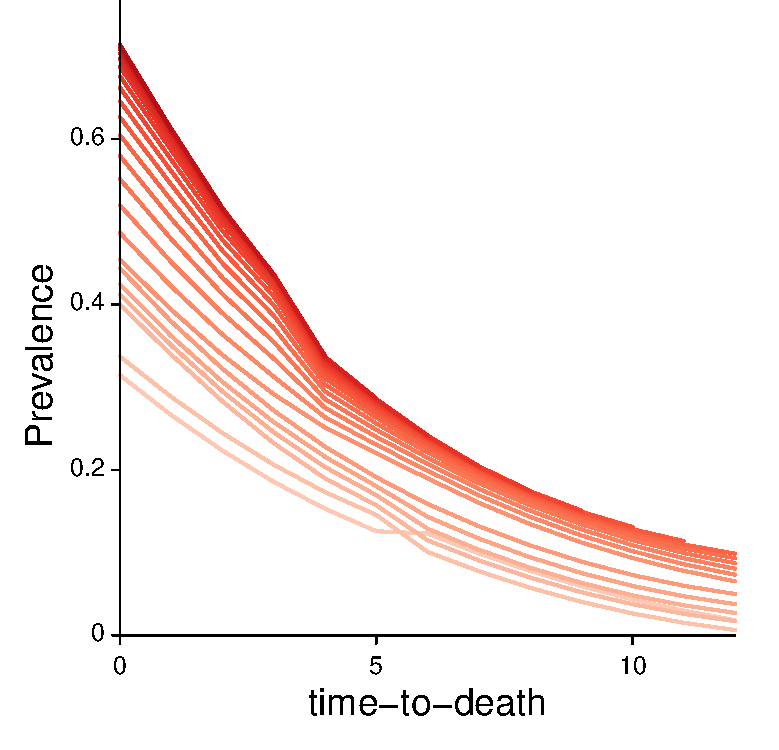
\includegraphics[scale=.8]{Figures/IADLttdlines.pdf}
\end{center}
\end{frame}

%%%%%%%%%%%%%%%%%%%%%%%%%%%%%%%%%%%%%%%%%%%%%%%%%%%%%%%%%%%%%
\section{How changing mortality affects morbidity prevalence}
%%%%%%%%%%%%%%%%%%%%%%%%%%%%%%%%%%%%%%%%%%%%%%%%%%%%%%%%%%%%%%

%%%%%%%%%%%%%%%%%%%%%%%%%%%%%%%%%%%%%%%%%%%%%%%%%%%%%%%%%%%%%%%%%%
\begin{frame}{Proportion disabled by TTD and mortality level}
%\begin{center}
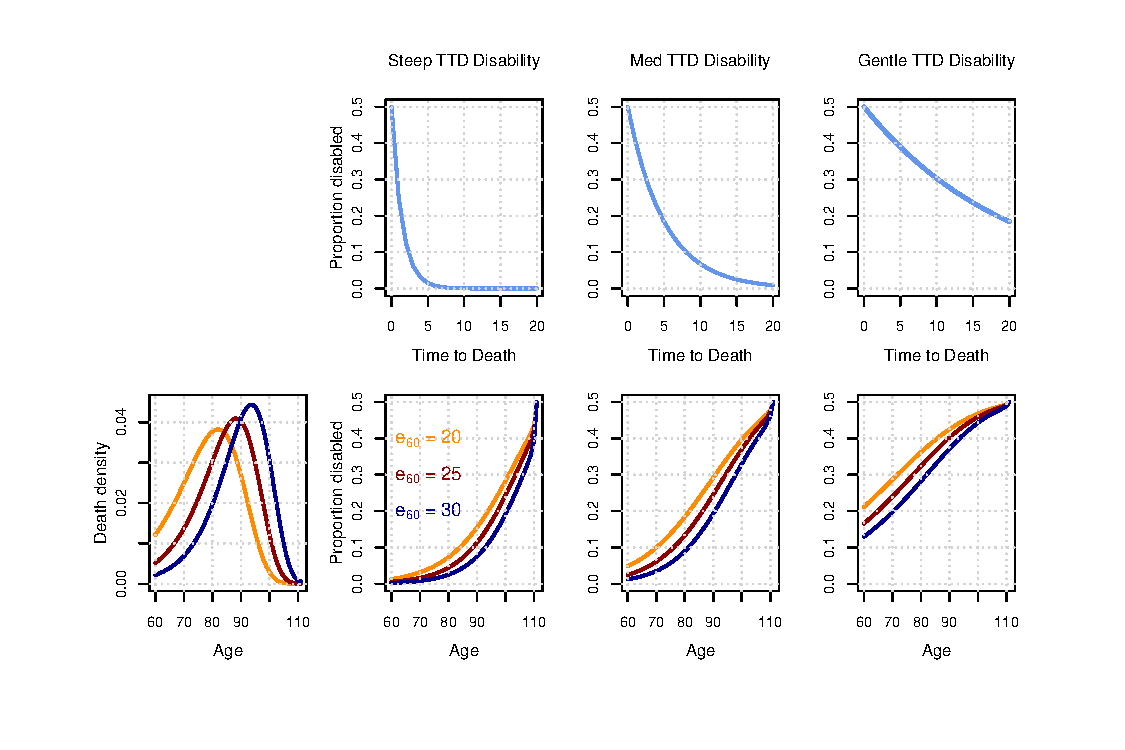
\includegraphics[trim=1cm 0 0 0, clip,
width=1.1\linewidth]{Figures/schematic_pres.pdf}
%\end{center}
\end{frame}
%%%%%%%%%%%%%%%%%%%%%%%%%%%%%%%%%%%%%%%%%%%%%%%%%%%%%%%%%%%%%%%%%%

%%%%%%%%%%%%%%%%%%%%%%%%%%%%%%%%%%%%%%%%%%%%%%%%%%%%%%%%%%%%%%%%
\section{Attributing DLY differences to mortality and morbidity}
%%%%%%%%%%%%%%%%%%%%%%%%%%%%%%%%%%%%%%%%%%%%%%%%%%%%%%%%%%%%%%%%

%%%%%%%%%%%%%%%%%%%%%%%%%%%%%%%%%%%%%%%%%%%%%%%%%%%%%%%%%%%%%%%%%%
\begin{frame}{Decomposing differences in DLY into mortality and morbidity}
\begin{itemize}[<+>]
\item Are differences in DLY from mortality or
morbidity?
\item Decomposition methods isolate the effects of changes in $L_x$ and changes
in $\pi_x$
\item These are considered as \textit{mortality} and \textit{morbidity} effects (Nusselder and Looman 2004, Andreev et al. 2002) 
\item Interpretation problem: mortality can change $\pi_x$ all by itself if
disability is patterned by time-to-death
\end{itemize}
\end{frame}
%%%%%%%%%%%%%%%%%%%%%%%%%%%%%%%%%%%%%%%%%%%%%%%%%%%%%%%%%%%%%%%%%%
\begin{frame}{Estimating the upper magnitude of bias of morbidity differences from mortality decline}
\begin{itemize}[<+->]
\item Estimated average TTD profile for different disability types, based on USA HRS data, quinquennial cohorts 1905-1930
\item Calculated apparent period age prevalence of morbidity for HMD countries had they experienced the US TTD morbidity 
\item Assumed all populations were stationary
\item Decomposed differences between all population pairs in 1980, 1990, 2000 into apparent mortality and morbidity components
\item Same for within-population changes over 10-year periods, 1950-2010
\end{itemize}
\end{frame}
%%%%%%%%%%%%%%%%%%%%%%%%%%%%%%%%%%%%%%%%%%%%%%%%%%%%%%%%%%%%%%%%%%%%%%%
\begin{frame}{TTD disability prevalence for different disabilty types}
\begin{center}
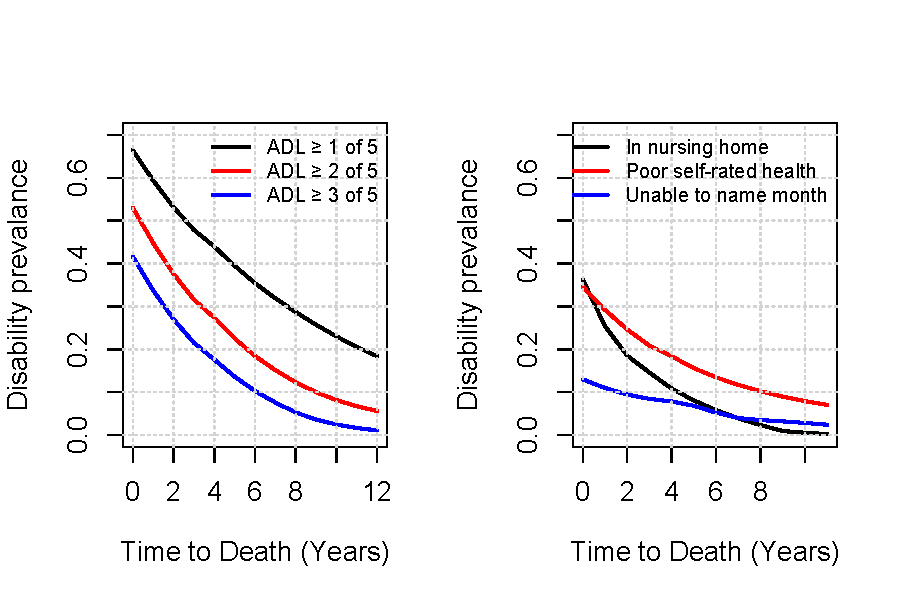
\includegraphics[scale=1.3]{Figures/DisbyTTD_pres.pdf}
\end{center}
\end{frame}
%%%%%%%%%%%%%%%%%%%%%%%%%%%%%%%%%%%%%%%%%%%%%%%%%%%%%%%%%%%%%%%%%%%%%%%
\begin{frame}{Decomposition: Change in disability component}
\begin{center}
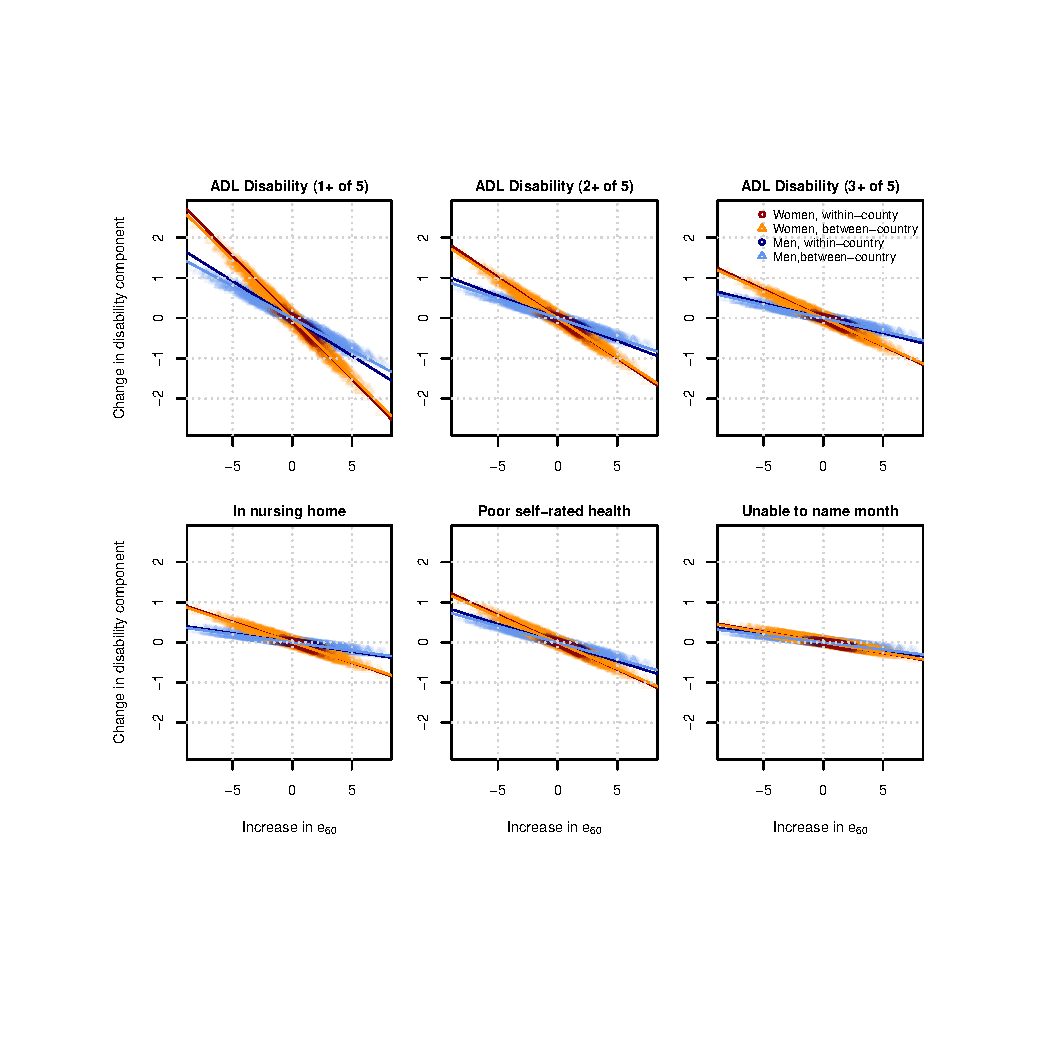
\includegraphics[trim=1cm 0 0 2.5cm, clip, scale=1.3]{Figures/Decomp_2x3.pdf}
\end{center}
\end{frame}
%%%%%%%%%%%%%%%%%%%%%%%%%%%%%%%%%%%%%%%%%%%%%%%%%%%%%%%%%%%%%%%%%%%%%%%%%
\begin{frame}{Interpreting decomposition results}
\begin{itemize}[<+>]
\item True value of the change in disability component is zero by design
\item Deviation is result of differences in mortality
\item If $e_{60}$ increases by 5 years, up to 1 year of decrease in DLY attributed to disability component could be from decrease in mortality (Female ADL 3 or more)
\item Departure from upper bound depends on patterns of $\pi_x$, how well US
pattern applies, departure from stationarity.
\item Different slopes partly from differences in final $\pi_x$ between
disability types and the sexes
\end{itemize}
\end{frame}
%%%%%%%%%%%%%%%%%%%%%%%%%%%%%%%%%%%%%%%%%%%%%%%%%%%%%%%%%%%%%%%%%%%%%%%%%%%%

%%%%%%%%%%%%%%%%%%%%%%%%%%%%%%%%%%%%%%%%%%%%%%%%%%%%%%%%%%%%%
\section{Conclusion}
%%%%%%%%%%%%%%%%%%%%%%%%%%%%%%%%%%%%%%%%%%%%%%%%%%%%%%%%%%%%%%

%%%%%%%%%%%%%%%%%%%%%%%%%%%%%%%%%%%%%%%%%%%%%%%%%%%%%%%%%%%%%%%%%%
\begin{frame}{Considerations}
\begin{itemize}[<+>]
\item Considering morbidity prevalence as a function of time to death does not imply that morbidity incidence is a time to death
\item Modeling prevalence as TTD requires no specification of process
\item In reality morbidity varies over both chronological age and time-to-death
\end{itemize}
\end{frame}
%%%%%%%%%%%%%%%%%%%%%%%%%%%%%%%%%%%%%%%%%%%%%%%%%%%%%%%%%%%%%%%%%%
%%%%%%%%%%%%%%%%%%%%%%%%%%%%%%%%%%%%%%%%%%%%%%%%%%%%%%%%%%%%%%%%%%
\begin{frame}{Summary}
\begin{itemize}[<+>]
\item HLE or DLY provide an important snapshot of expected life years lived in good or poor health
\item Difficulty in interpreting period differences in these quantities between populations 
\item Chronological age pattern of disability can change solely as a function of mortality change even when the underlying morbidity function is held constant
\item Could partly explain why mortality levels and disability prevalence are related (Van Oyen et al. 2013, Luy and Minagawa 2014)
\end{itemize}
\end{frame}
%%%%%%%%%%%%%%%%%%%%%%%%%%%%%%%%%%%%%%%%%%%%%%%%%%%%%%%%%%%%%%%%%%



%%%%%%%%%%%%%%%%%%%%%%%%%%%%%%%%%%%%%%%%%%%%%%%%%%%%%%
%\begin{frame}[plain]
%\begin{center}
%\huge Thank you for you attention \\
%\vspace{0.5cm}
%\normalsize riffe@demogr.mpg.de\\ 
%\normalsize vanraalte@demogr.mpg.de\\ 
%
%\end{center}
%\end{frame}

\begin{frame}
\frametitle{Thanks!}
\begin{center}
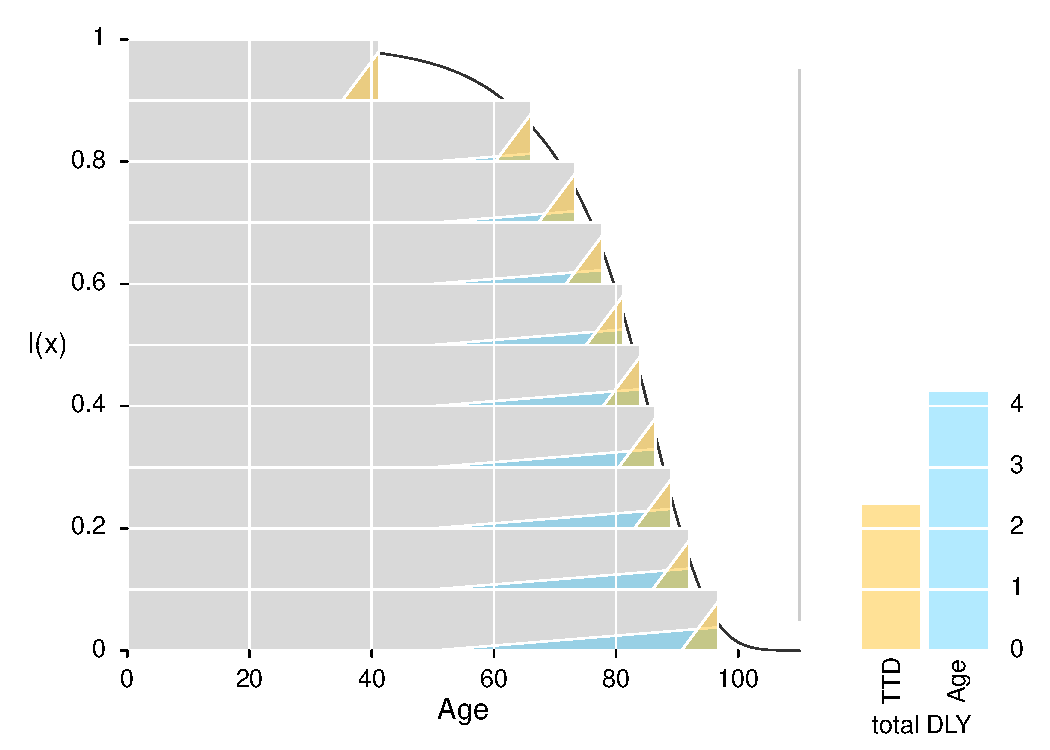
\includegraphics[width=\linewidth]{Figures/Japan2010.pdf}
\end{center}
\end{frame}

%%%%%%%%%%%%%%%%%
\end{document}